\section{Introduction}
\label{sec:intro}

\begin{figure}[t]
\centering
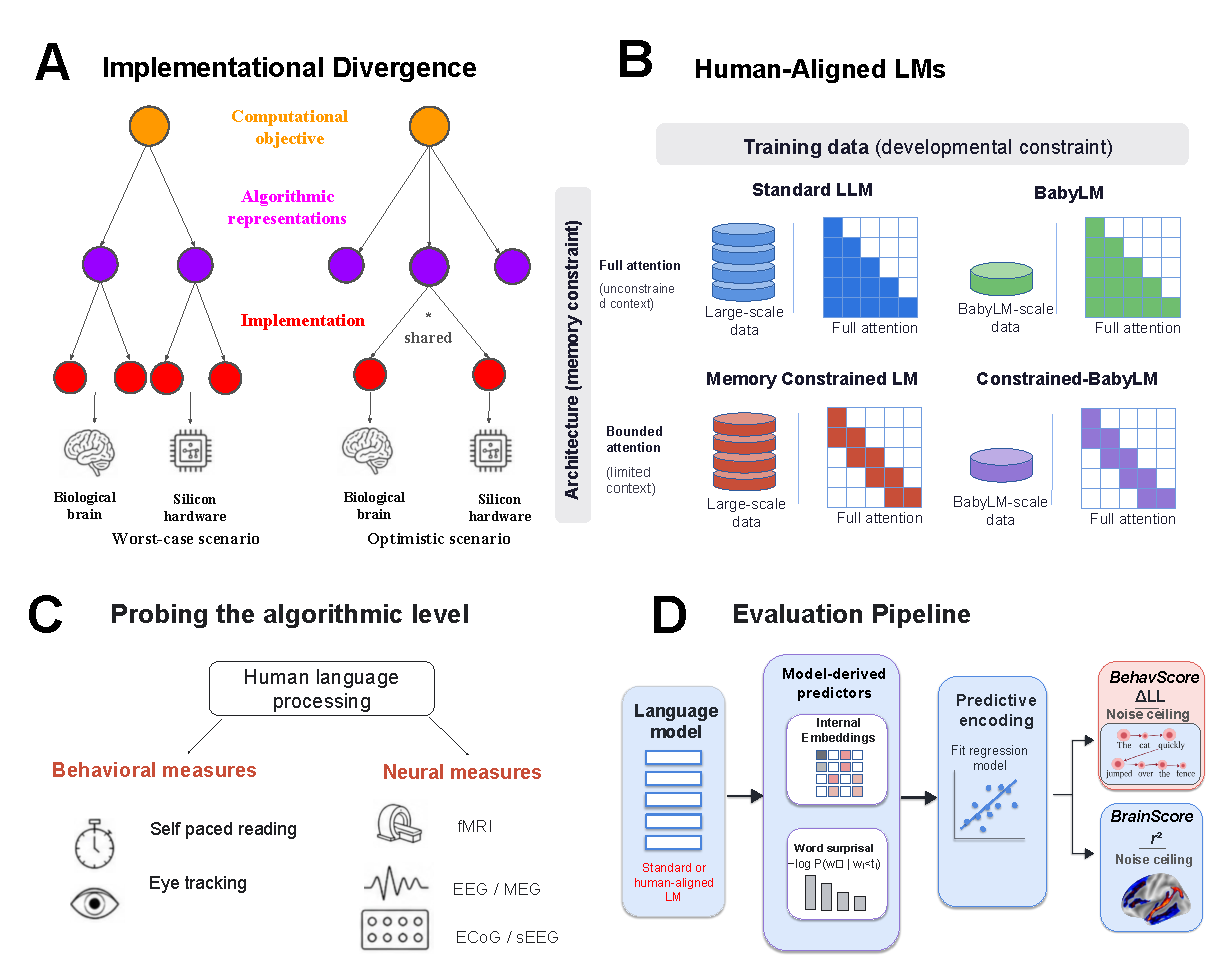
\includegraphics[width=\textwidth]{figures/figure1_overview.pdf}
\caption{Overview of the study. (A) Marr's tri-level framework applied to humans and LLMs: even where the two systems share the same algorithmic-level representations (optimistic scenario), they may still diverge at the computational and implementational levels. (B) Human-aligned language models introduce either architectural constraints (limited attention, memory decay) or data constraints (developmentally limited training exposure) relative to standard LLMs. (C) Human language processing is probed through behavioral measures (self-paced reading, eye-tracking) and neural measures (fMRI, EEG/MEG, ECoG). (D) Final-layer LLM predictors, internal representations and word surprisal, are used to predict held-out behavioral and neural data (BehavScore and BrainScore), and are complemented by representational comparisons. Neither kind of correspondence alone establishes a shared algorithm.}
\label{fig:overview}
\end{figure}

Do humans and Large Language Models (LLMs) process language in a similar way? David Marr's tri-level framework provides a principled lens for this question by decomposing information-processing systems into three levels (Figure~\ref{fig:overview}A): the computational level (what is the goal of the computation?), the algorithmic level (what representations and step-by-step procedures are used?), and the implementational level (how are these steps physically realized?) \citep{marr1982vision}. At the computational level, LLMs are primarily optimized for next-word prediction over massive text corpora. While predictive processing plays a central role in human language comprehension \citep{hale2001probabilistic,levy2008expectation,smithlevy2013effect,shain2024large}, next-token prediction is at best a rough proxy: biological language processing is also driven by communicative intent, pragmatic inference, multi-step predictive horizons, and social or goal-directed rewards \citep{bender-koller-2020-climbing,andreas-2022-language}. At the implementational level, the differences are clearer still. Standard LLMs rely on global self-attention over long context windows \citep{vaswani2017attention}, uniform stacks of Transformer blocks that lack the modular organization of the cortical language network, non-local backpropagation rather than local learning rules, and training exposure spanning trillions of tokens, orders of magnitude beyond a human lifetime \citep{gilkerson2017mapping,warstadt2023cfp}.

Given these differences at the computational and implementational levels, do LLMs and humans converge on similar representations and processing steps at the algorithmic level? At one extreme, the mismatches drive LLMs and human brains to adopt fundamentally different procedures. At the other, aligned with the Platonic Representation Hypothesis \citep{huh2024platonic}, shared environmental pressures and task demands push biological and artificial systems toward the same representations despite their structural differences. Which of these outcomes holds, and for which aspects of language processing, remains an open empirical question.

Cognitive scientists and neuroscientists have responded by building models that incorporate explicit human constraints, with the aim of moving them closer to human processing at the algorithmic level. On the architectural side, models introduce human cognitive limitations such as working-memory bottlenecks \citep{lewisvasishth2005activation}, lossy or decaying context \citep{futrell2020lossy}, recurrent processing dynamics \citep{michaelov2024revenge}, or localized attention \citep{devarda2024locally,kuribayashi2022context}. On the data side, initiatives such as the BabyLM Challenge restrict training to developmentally realistic, child-scale input of 10 to 100 million words rather than web-scale text (Figure~\ref{fig:overview}B; \citealp{warstadt2023cfp,warstadt2023findings}). These choices change the information available to a model and the representations it can learn. Whether they produce closer correspondence with human data, or whether standard LLMs already achieve comparable correspondence through scale, is an empirical question.

In humans, the algorithmic steps of language processing are probed through behavioral and neural measures (Figure~\ref{fig:overview}C). Behavioral measures such as self-paced reading times and eye-tracking fixations index moment-by-moment processing difficulty \citep{futrell2021natural,frank2013reading,luke2018provo,siegelman2022meco}. Neural measures capture complementary spatio-temporal scales: fMRI provides whole-brain spatial coverage \citep{schrimpf2021neural}; EEG tracks temporal dynamics such as the N400 \citep{michaelov2024strong,federmeier2007multiple}; MEG and intracranial recordings combine finer temporal resolution with, for the latter, direct cortical access. A model that captures variation in reading difficulty need not be the model that most closely matches neural responses. This distinction matters when evaluating human-inspired models: a constraint intended to approximate human memory or training exposure may improve one aspect of alignment without improving another. Rather than interpreting model internals in isolation, we ask how well model-derived features, word surprisal and contextual embeddings, predict human behavioral and neural responses, and how closely the representational geometry of the model matches that of the responses (Figure~\ref{fig:overview}D).

We test these questions in a $2\times2$ design that crosses an architectural memory constraint with a developmental data constraint: (1) memory-constrained architectures trained at web scale, (2) the same architectures trained on BabyLM-scale data, (3) standard architectures trained on BabyLM-scale data, and (4) standard, off-the-shelf LLMs with neither constraint. We evaluate 118 frozen models on 18 datasets spanning self-paced reading, eye-tracking, fMRI, EEG and N400 responses, MEG, and intracranial recordings, using final-layer embeddings and surprisal as predictors. We first identify individual models that offer competitive combinations of behavioral and neural prediction, using Pareto fronts. Because the four groups differ by orders of magnitude in parameter count and language-modeling quality, we then estimate group associations separately for behavioral and neural outcomes, adjusting for parameter count and perplexity. Finally, we compare direct prediction with unfitted representational similarity analysis (RSA) and confound-controlled regression on representational dissimilarity matrices (RDMs).

The central result is a behavioral--neural distinction. For contextual embeddings, data-constrained models predict reading behavior better than size- and perplexity-matched standard LLMs, but not neural responses, while memory-constrained models predict neural responses worse; both domain differences are tested directly and survive modeling the dependence between related models, a lineage cluster bootstrap, and dataset exclusions. Combining the two constraints cancels the behavioral advantage. Surprisal-based constraint effects are weaker and depend on datasets with unstable noise ceilings. Size also has different associations across outcomes: larger models have higher neural embedding scores, whereas behavioral surprisal prediction declines with size conditional on perplexity. Representational evaluations reinforce the competitiveness of small and constrained models for behavior, while revealing that neural rankings depend on the scoring method.

We use \emph{alignment} to denote these measured correspondences. Correspondence in predictions or representational geometry can inform models of cognition without identifying a shared algorithm \citep{marr1982vision}. Our contribution is therefore a comparative account of where constraints are associated with closer correspondence to human data, rather than a single verdict on whether constrained or standard language models are more human-like. Specifically:
\begin{itemize}
    \item We evaluate 118 language models from four constraint groups on 18 behavioral and neural datasets (27 dataset units) with both embedding and surprisal predictors, under one common pipeline, and release it as the HumanScore-Language benchmark.
    \item We separate the association of each human-inspired constraint from that of model size and perplexity, with separate analyses for behavioral and neural responses and an explicit test of the interaction between the two constraints.
    \item We show, with inference that accounts for the dependence between related models and datasets and directly tests the difference between domains, that a developmental data budget is associated with better behavioral but not neural prediction and a memory constraint with worse neural prediction, and that their combination is not additive.
    \item We show that model rankings differ between direct prediction, unfitted RSA, and confound-controlled RDM regression, so that no single evaluation suffices to rank models by human-likeness.
\end{itemize}
